\documentclass[%
reprint,
%linenumbers,
superscriptaddress,
amsmath,amssymb,showkeys,
aps,
prb,
]{revtex4-2}
\usepackage[T1]{fontenc}
\usepackage{graphicx}% Include figure files
\usepackage{dcolumn}% Align table columns on decimal point
\usepackage{bm}% bold math
\usepackage{physics}
\usepackage[sort&compress]{natbib}
\usepackage{ulem}
\usepackage{url}
\usepackage{hyperref}
\usepackage{bbm}

\begin{document}
	\preprint{APS/123-QED}
	
	\title{Time Crystal Embodies Chimera in Periodically Driven Quantum Spin System}
	
	\author{Mahbub Rahaman}
	\thanks{Primary and corresponding author}
    \email[\\Email: ]{mrahaman@scholar.buruniv.ac.in}
	\affiliation{Department of Physics, The University of Burdwan, Burdwan 713104, India}	
	\author{Akitada Sakurai}
	\affiliation{Quantum Information Science and Technology Unit, Okinawa Institute of Science and Technology Graduate University, Onna-son, Okinawa 904-0495, Japan}		
	\author{Analabha Roy}
	\thanks{Co-corresponding author}
    \email[\\Email: ]{daneel@utexas.edu}
	\affiliation{Department of Physics, The University of Burdwan, Burdwan 713104, India}

	\begin{abstract}
		Chimera states are a captivating occurrence in which a system comprised of multiple interconnected elements exhibits a distinctive combination of synchronized and desynchronized behavior. The emergence of these states can be attributed to the complex interdependence between quantum entanglement and the delicate balance of interactions among system constituents. The emergence of Discrete Time Crystal (DTC) in typical many-body periodically driven systems occurs when there is a breaking of time translation symmetry. Coexisting coupled DTC and a ferromagnetic dynamically many-body localized (DMBL) phase at distinct regions have been investigated under the controlled spin rotational error of a disorder-free spin-1/2 chain for different types of spin-spin interactions. We contribute a novel approach for the emergence of the DTC-DMBL-Chimera phase, which is robust against external static fields in a periodically driven quantum many-body system.
	\end{abstract}
	
	\keywords{Dynamical Many Body localization, Chimera in a quantum system, Time crystal, Periodic drive.}
	\maketitle
	
	Symmetry is a fundamental concept in physics. It provides insight into finding the conservation laws, establishing new theories, such as a gauge theory~\cite{Yang_1954}, and understanding the many-body physics. In condensed matter physics, symmetry and its breaking (spontaneous symmetry breaking or SSB) play an essential role in formulating the phases of matter. SSB has been seen at different scales, such as the Higgs mechanism in high-energy physics, cosmology, and Bose-Einstein condensation in cold atoms, etc. ~\cite{krasnov_spontaneous_2012, sadler_spontaneous_2006, vanderbruggen_spontaneous_2015}.
	
	In solid-state physics, a state shows crystalline order due to continuous translational symmetry breaking in space. Motivated by the equivalence between space and time in relativistic theory, one can consider SSB along the time axis and a new phase of matter in the temporal axis. Frank Wilczek proposed a framework in 2012 on  $\textit{time translation symmetry breaking}$ (TTSB) in quantum mechanical systems ~\cite{wilczek_quantum_2012}. In another paper, Shapere and Wilczek proposed TTSB for a classical system~\cite{shapere_classical_2012}. This unveils a new state of matter, $\textit{Time Crystals}$ (TC), where the ground state of the system possesses its own dynamics, distinct from external influence~\cite{wilczek_quantum_2012}, which arises from the intrinsic properties and interactions among the system constituents. Additionally, to sustain the periodicity of the TC, the necessary energy originates from external fields. Wilczek's proposed TC was an equilibrium state of matter where continuous time translation symmetry was broken. Later, Oshikawa and Watanabe proved that the TC cannot exist in a thermal equilibrium system (\textit{the no-go theorem}) ~\cite{watanabe_absence_2015}. Their proof does not reject the possibility of the TC  existing in a non-equilibrium system, such as Floquet systems. Hence, the Floquet time crystal (or Discrete time crystal(DTC)) was proposed, in which discrete, not continuous symmetry is broken~\cite{else_floquet_2016}.
	
	In a generic DTC, a strong disorder is applied, which results in many-body localization (MBL) in the system in a controlled fashion. This prevents DTC from undergoing a thermalization by exchanging energy with heat-bath (or by sub-system of the closed system)~\cite{alet_many-body_2018,else_floquet_2016,smith_many-body_2016,nguyen_signature_2021}. The introduction of MBL sustains the DTC order to survive for a sufficiently long time ~\cite{zhang_observation_2017}. Direct quenches, Delta-Kicks, and other periodic driving methods are also widely used to construct DTCs~\cite{else_prethermal_2017, russomanno_spin_2017, ho_critical_2017, yu2019, russomanno_floquet_2017}. These methods do not need the application of disorder. DTCs have been experimentally realized in several different many-body systems, such as an array of ion trapped interacting spins~\cite{huang2018,taheri_all-optical_2022, Soham2018, zhang_observation_2017, yao_time_2018,sacha_modeling_2015}, qubits ~\cite{frey_realization_2022}, ordered dipolar $NH_4H_2PO_4$~\cite{rovny_observation_2018}, bouncing ultracold atoms on oscillating mirror~\cite{sacha_time_nodate,golletz_basis_2022} etc. Recent works corroborate the emergence of disorder-free dynamical many-body localization(DMBL) through system dynamics by applying an external periodic drive~\cite{Keser2016, haldar_dynamical_2017, haldar_dynamical_2021,bhattacharyya_transverse_2012,aditya2023dynamical,dutta2014,das_exotic_2010} which is another prospect in the construction of a stable DTC.
	
	In classical systems, the coexistence of coupled spontaneous synchronized and desynchronized system dynamics emerges in coupled identical oscillators. This is called \textit{Chimera}~\cite{kuramoto_coexistence_2002, panaggio_chimera_2015, parastesh_chimeras_2021}. The idea of chimera was brought into quantum systems, and the Chimera order has been investigated as a quantum phase of matter~\cite{bastidas_quantum_2015}. In recent decades, a new chimera order has been found in a quantum spin system \textit{s.t.} \textit{Ising model-chimera}, where coexisting ordered and disordered phases are detected through magnetization~\cite{singh_chimera_2011}.  
	
	In this article, we investigate if a chimera consisting of a DTC and a localized ferromagnetic state can coexist simultaneously in a one-dimensional spin-1/2 chain driven by external drives. Recent advancements in this domain involve the formation of a \textit{chimera time crystalline order}, as reported by Sakurai et al.~\cite{sakurai_phys_nodate} performed by the application of disorder in a one-dimensional interacting spin-1/2 chain. In this paper, we have employed a periodically driven transverse field that breaks $\mathbb{Z}_2$ symmetry by system-dynamics in a one-dimensional \textit{disorder-free} quantum spin-1/2 chain and incorporates a power-law decay Heisenberg spin exchange interaction.
	
	The article is presented as follows: In the section~\ref{sec:mdl_n_dynam}, the proposed spin model and system dynamics are described. In the section~\ref{sec:level2}, we describe the emergence of DMBL. In section ~\ref{sec:level3}, we numerically investigate the coexistence of the time crystal and a DMBL phase, supported by an analytical approach. In section ~\ref{sec:level4}, regional magnetization and  entanglement entropy for the system are investigated, and in section~\ref{sec:level6} we explore the robustness of the system against the external static field. Finally, we discuss our results and conclude.	
	
	\section{\label{sec:mdl_n_dynam} The Model and System Dynamics}
	We consider a one-dimensional spin-1/2 chain with N sites. In the chain, all sites are connected via the Heisenberg interaction. We divide the chain into two regions denoted as regions $A$ and $B$, and these regions are under the time-periodic driving. The system's Hamiltonian is time-periodic with a period $T=T_1+T_2$, and is given by,
	
	\begin{align}
		\hat{H}(t) = 
		\begin{cases}
			\hat{H_1} , & 0\leq t < T_1,\\
			\hat{H_2} , & T_1\leq t < T,
		\end{cases}
		\label{eq:cleanham}
	\end{align}
	where,
	\begin{align}
		\hat{H_1} = & \hbar g (1-\epsilon_A) \sum_{\substack{\\i \in A}}\hat{\sigma}^x_i + \hbar g (1-\epsilon_B) \sum_{i \in B}\hat{\sigma}^x_i+ \hbar\hat{V}(\hat{\sigma}^{\gamma}),\label{eq:sysham1}\\
		\hat{H_2} = & \hbar\sum_{ij} J_{ij} \hat{\sigma}^y_i \hat{\sigma}^y_{j} +  \hbar h_D \sum_i \hat{\sigma}^z_i + \hbar\hat{V}(\hat{\sigma}^{\gamma}),
		\label{eq:sysham2}
	\end{align}
	where $\hat{\sigma}^{\mu=x,y,z}_i$ are the Pauli matrices at $i$-th site, and $T_2 = T-T_1$, such that $T_1=T_2=T/2$. 
	
	The first two terms of the Hamiltonian $\hat{H}_1$ in Eq.\eqref{eq:sysham1} represent the periodic driving with a strength $g$. To realize the DTC phase on the chain, we set $g=\pi/T$, which causes a spin flip. Here parameters $\epsilon_{A/B}\in[0,1]$ are rotational errors for two regions. These two parameters play an essential role in making the difference between the two regions. For instance, when $\epsilon_A \sim 0$ and $\epsilon_B \sim 1$, the driving in region-A is imperfect spin flip, while that in region-B is not. The third component can be expressed as $\displaystyle \hat{V}(\hat{\sigma}^{\gamma}) =\gamma  \sum_{i=1}^{N} (\hat{\sigma}^x_i + \hat{\sigma}^y_i)$ which serves as a controlled additional static field that operates in the $x$ and $y$ spin axes and can also be interpreted as a static magnetic imperfection that is modulated by a parameter $\gamma$.
	
	The second Hamiltonian $\hat{H}_2$ in Eq.\eqref{eq:sysham2} represents a chain where two sites are coupled and all sites are under two different potentials. Its first term is the interaction between two sites$(i>j)$ with a coupling strength $J_{ij}$. In this paper, we assume that the strength follows the power law decay and can be written as $J_{ij}={J_0}/{|i-j|^\beta}$ with coupling constant $J_0$.
	Exchange energy per spin decays as $\beta$ increases. We have adapted Buyskikh's benchmarking ~\cite{buyskikh_entanglement_2016} to classify the scaling of spin-spin interaction by varying $\beta$. When $\beta$ takes the value ranges in  $0 \leq \beta <1$ the interaction is classified as \textit{long-range} or \textit{all-to-all} interaction; $1<\beta<2$ it is \textit{intermediate-range} interaction; $\beta > 2$ is considered as \textit{short range} and when $\beta= \infty$ the interaction is called \textit{nearest neighbor} range.
	
	
	Next, the second term in $\hat{H}_2$ is a continuous transverse time-periodic drive $\displaystyle \hat{H}_D=\hbar h_D \sum_i\hat{\sigma}^z_i$, where $\displaystyle h_D = -h\sin{(\omega t)}$ considering $h$ and $\omega$ are the amplitude and frequency of the drive. We have considered $\omega$ to be sufficiently high such that $\omega\gg J_0$. At specific values of $h$ and $\omega$, our model shows a dynamical state that facilitates the manifestation of DMBL, which prevents the system from rapid thermalization. Later in section\ref{sec:level2}, we will discuss this point in detail. 
	The third constituent of the Hamiltonian $\hat{H_2}$ is the static magnetic imperfection, which is $\displaystyle{\hbar\hat{V}(\hat{\sigma}^{\gamma})}$. 
	
	In this paper, we have initially fixed $\hat{V}(\hat{\sigma}^\gamma)=0$ and investigated the realization of the proposed chimera. Later in section\ref{sec:level6} we introduced finite values of $\hat{V}(\hat{\sigma}^\gamma)$ to investigate the robustness of the chimera in the presence of the additional external static magnetic field.
	
	\begin{figure}
		\centering
		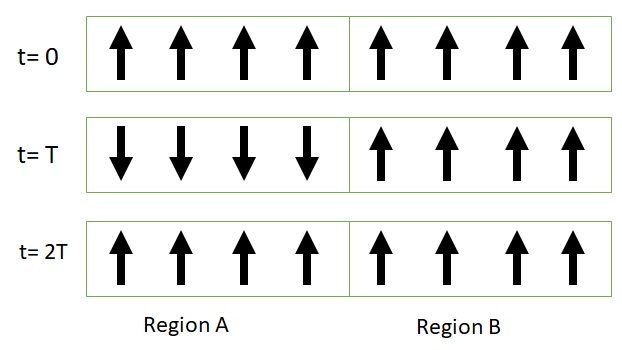
\includegraphics[width=7.0cm]{pic_regions.jpg}
		\caption{Changes in spin orientation in the bipartite spin1/2 chain are featured for regions A and region B at time $t= 0, T, 2T$. Spins at region B remain unaltered for all time. In region A, spins experience spin-flip at T, manifesting a \textit{period-doubling} in Region A at 2T.}
		\label{Fig:spinflip}
	\end{figure}
	
	At the outset, it is postulated that the spins exhibit polarization exclusively in the spin-up orientation. During $T_1$ the spins located within region A, undergo a \textit{spin-flip} resulting in a spin-down orientation, while the spins situated within region B, remain in spin-up orientation as in Fig.~\ref{Fig:spinflip}. There is no spin-spin interaction term except a spin alteration periodic drive in $\hat{H}_1$. This keeps the spins localized in region A at each spin-flip operation via quantum tunneling destruction. In $T_2$ time interval, a periodically driven transverse field is globally applied to the spin chain, such that both regions A and B experience DMBL. If the system is driven up to the next time period 2T, a spin magnetization \textit{period doubling}~\cite{rovny_31mathrmp_2018, Pan2020} is expected. Experimentally, it can be performed using external driving with high frequency to the Hamiltonian $\hat{H}_2$, in which, in other words, its time scale is much shorter than that of interactions.~\cite{choi_observation_2017,zhang_observation_2017,Cirac_1995,Blatt_2012}
	
	\section{\label{sec:level2} Interacting Dynamical Localization}
	
	Before investigating the chimera order in our model, let us explain that the Hamiltonian $\hat{H}_2$ in Eq.~\eqref{eq:cleanham} shows the Dynamical Many-Body Localization (DMBL). We investigate DMBL analytically for $T_2$  when the system is driven by a sinusoidal transverse periodic drive $h_D$ in $\hat{H}_2$ as illustrated in Fig.~\ref{Fig:time_distribution}.
	\begin{figure}
		\begin{center}
			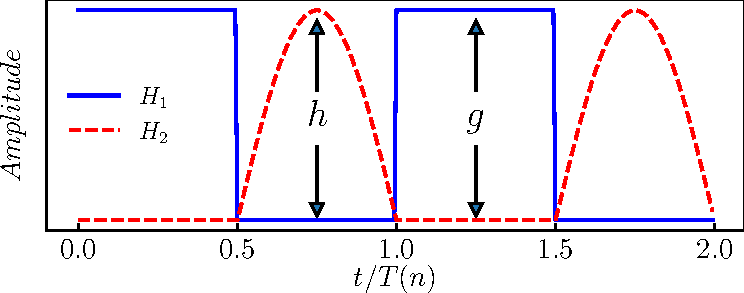
\includegraphics[width=7.5cm]{drive_distribution.pdf}
		\end{center}
		\caption[]{Pictorial realization of the temporal progression of external drive for two time periods. The drive is considered in such a way that a spin-flip constant drive $\hat{H_1}$ acts during $T_1$(blue curve) and the periodic drive part of $\hat{H_2}$ in $T_2$(red dashed curve). The ordinate is amplitude and abscissa denotes n'th time period.}
		\label{Fig:time_distribution}
	\end{figure}	
	We have the employed the \textit{moving frame method}~\cite{haldar_dynamical_2021}, where a unitary transformation operator is operated to transform the Hamiltonian into a reduced form. The transformation evolution operator $\hat{U}$ reduces the state $\ket{\psi(t)}$ into a mobile frame in time $t$ as $\ket{\psi(t)}_{mov} = \hat{U}^\dagger \ket{\psi(t)}$, where $\hat{U}$ can be expressed as the time-varying constituent of the Hamiltonian,
	\begin{equation}
		\hat{U}(t) = e^{-\frac{i}{\hbar}\int_{0}^{t} dt' \hat{H}_D}.
		\label{eq:rot1}
	\end{equation}
	The unitary transformation operator for the Hamiltonian $\hat{H_2}$ for the time interval $T_2$, $\in{\Big[\frac{T}{2}, (\frac{T}{2}+t) \Big]}$ is,
	\begin{align}
		\hat{U}(t) =& \exp \Bigg[-\frac{i}{\hbar}\int_{\frac{T}{2}}^{\frac{T}{2}+t} (-h \sin(\omega t'))dt'\hbar\sum_i\hat{\sigma}^z_i\Bigg]\nonumber\\
		=& \prod_{i} \exp\Big[-i \hat{\sigma}^z_i\xi(t))\Big],
	\end{align}	
	where, $\displaystyle{
		\xi (t) = h\int_{\frac{T}{2}}^{\frac{T}{2}+t}  \Big[-\sin(\omega t')dt'\Big]=  \frac{h}{\omega}\Big[1-\cos(\omega t)\Big]}$.		
	Now, in the rotating frame, the Hamiltonian can be written as~\cite{haldar_dynamical_2021},
	\begin{align}
		\hat{H}^{mov} &= \hat{U}^\dagger(t) \hat{H}(t) \hat{U}(t)- i \hat{U}^\dagger(t) \partial_t \hat{U}(t)\nonumber\\
		&= \hat{U}^\dagger(t) \big[\hbar\sum_{ij}J_{ij}\hat{\sigma}^y_i\hat{\sigma}^y_j\big] \hat{U}(t)\nonumber\\
		&=\hbar\sum_{ij} J_{ij} \Big(\hat{\sigma}^y_i\hat{\sigma}^y_j\Big) e^{i 2\xi \hat{\sigma}^z_i}  e^{i 2\xi \hat{\sigma}^z_j}
		\label{eq:movham}
	\end{align}
	We have applied Jacobi Anger expansion, $\displaystyle e^{iz \cos(\theta)} = \sum_{n=-\infty}^{\infty} \mathcal{J}_n(z) e^{in\theta}$, where $\mathcal{J}_n$'s denote the roots of the Bessel's function of first kind of $n$'th order. We can neglect the high-order terms due to the high-frequency external drives. Considering only the zeroth order term, the transformed Hamiltonian Eq.\eqref{eq:movham}reduces to,
	\begin{multline}
		\hat{H}^{mov} =\hbar \sum_{ij} J_{ij} \Big(\hat{\sigma}^y_i\hat{\sigma}^y_j\Big)J_0\Big(\frac{4h}{\omega}\Big) \\\Bigg[\cos[2](\frac{2h}{\omega}) -i\Big(\hat{\sigma}^z_i\hat{\sigma}^z_j\Big) \sin[2](\frac{2h}{\omega})\\+ i (\hat{\sigma}^z_i + \hat{\sigma}^z_j)\cos(\frac{2h}{\omega})\sin(\frac{2h}{\omega})\Bigg]
		\label{eq:movham1}
	\end{multline}
	Now, if the drive parameters $h$ and $\omega$  are varied in such a way that the ratio, $({4h}/{\omega})$ lies at one of the roots of $\mathcal{J}_0$, it is possible to nullify the effective Hamiltonian $\hat{H}^{mov}$ which localizes the system during $T_2$. The Eq.\eqref{eq:movham1} describes the necessary condition for emergence of DMBL during $T_2$. This is supported by the numerical results in section~\ref{sec:level42}, where $\hat{\sigma}^z$ is detected as an existing integral of motion as $M^Z_B$ for region-B remains constant unity and independent of time, which confirms a DMBL~\cite{Keser2016,Dodonov1978}. 
	
	
	\section{\label{sec:level3}Coexistence of DTC \& DMBL}
	
	To see the emergence of the chimera state in our model, we will numerically calculate the local magnetization,$\left\langle{\hat{S}^z}\right\rangle_i = \expval{\hat{\sigma}^z_i}{\Psi(t)}$ of spin chain, for sufficiently longer time (up to 80 periods) for different $\beta = 0,1.5,2.5,\infty$ and different interaction strengths, weak($J_0 = 0.2/T$) and strong ($J_0 = 0.072/T$), following Sakurai's work~\cite{sakurai_phys_nodate}. To investigate the rigidity of our model, we set the rotational error $\epsilon_A = 0.03$, $\epsilon_B = 0.9$. Additionally, to see the emergence of the chimera state in our model, we consider periodic drive at $\hat{H}_2$ with high frequency $\omega=20$ for both cases where $\mathcal{J}_0(\varpi)$ with $\varpi = 4h/\omega$ is at the roots of $\mathcal{J}_0$ \textit{i.e.} the DL point and away from it. The results are shown in Fig.~\ref{Fig:strong_weak_ea}. 

    \begin{figure*}[t!]
		\centering
		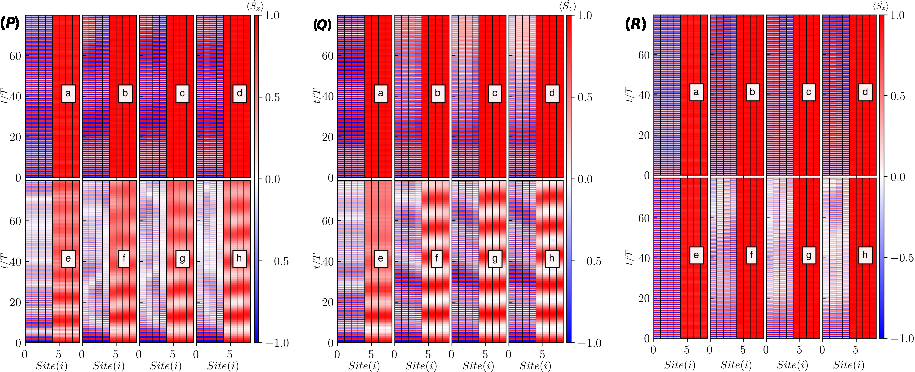
\includegraphics[width=17.5cm]{sz_t_strongweakJ_ea_N_8.pdf}
		\caption{The time evolution of local magnetization for each spin at region A (Site(i)=0,1,2,3) and region B (Site(i)=4,5,6,7) is plotted for up to 80T, taking spin rotation error $\epsilon_A = 0.03$ and $\epsilon_B = 0.9$ with $g=\pi/T$.  In all three panels P, Q, and R, different spin-spin interactions such as long-range, intermediate range, short range, and nearest neighbor range are taken into account and plotted respectively from left to right, namely, (a, b,c,d) in the top row and (e,f,g,h) in the bottom row of each panel. The time evolution considering strong spin coupling ($J_0 = 0.2/T$) in the left panel (P) and weak spin coupling ($J_0 = 0.027/T$) in the middle panel (Q) is plotted  for the DL point (top panels of P \& Q) and away from the DL point (bottom panels of P \& Q). In the right panel (R), local magnetization for an effectively small spin rotational error $\epsilon_A = 0.05$ (top panel of R) and a larger $\epsilon_A = 0.1$ (bottom panel of R) are plotted at the DL point. At small $\epsilon_A=0.5$, the DTC-DMBL chimera is stable, while at $\epsilon_A=0.1$, DTC is stable only for long-range interaction, but in other spin ranges, the DTC phase melts at larger times.}
		\label{Fig:strong_weak_ea}
	\end{figure*}
	
	As shown in Fig.~\ref{Fig:strong_weak_ea}, at the DL points with strong coupling, the local magnetization for all types of spin-spin interaction shows periodic dynamics with double periods ($2T$) of the driving in region A, while that of region B is stable in time. Thus, regions A and B are the DTC and DMBL phases respectively. It indicates that two different phases of matter coexist in the same spin chain. Thus a chimera state emerges. In contrast, the system dynamics is unstable away from the DL point for both values of $J_0$. Similarly, in the weak interaction, the long-range $(\beta=0.0)$ shows stable DTC and DMBL phases. However, for intermediate($\beta = 1.5$), short-range ($\beta = 2.5$), and nearest neighbour range ($\beta = \infty$) interactions, DTC melts in a short period ($\sim$ 20 periods) in region A. These results are in agreement with previous work~\cite{sakurai_phys_nodate}.
		
	The stability of the DTC phase exhibits notable disparities between strong and weak coupling interactions. Specifically, even at the DL point, the DTC phase demonstrates greater stability in the presence of strong coupling as compared to weak coupling for interactions other than long-range interaction. The long-range interaction persists in a stable DTC for both strong and weak spin interactions. Thus the spin chain constitutes two existing simultaneous distinct phases of matter, a DTC and a ferromagnetic localized phase coupled together, manifesting a \textit{chimera} in the quantum spin chain. So in general, long-range coupling is the best candidate for constructing a DTC-ferromagnetic(DTC-DMBL) chimera.
	
	In addition, higher values of $\epsilon_A$ are applied to investigate the stability of DTC against larger rotational errors (see Fig.~\ref{Fig:strong_weak_ea}(R)). We have considered $\epsilon_A = 0.05$  and $0.1$ at fixed $\epsilon_B = 0.9$ for $\beta = (0.0, 1.5, 2.5, \infty$), fixed at DL points at strong coupling($J_0 = 0.2/T$). At a small $\epsilon_A=0.05$, DTC is stable for all types of spin-spin interactions. At large $\epsilon_A = 0.1$, the long-range($\beta=0$) DTC is stable, though, for other types of spin-spin interaction, DTC vanishes very fast, even after a couple of time periods. This corroborates the proffer that long-range interaction are the best choice for constructing a DTC-DMBL-chimera. 
	
	Next, to further investigate the DTC and DMBL phases coexisting further, let us consider the \textit{Floquet theory}, which is used to analyze the dynamics at the stroboscopic times. The effective Floquet Hamiltonian for two periods is given by,
	\begin{widetext}
		\begin{multline}
			H^{\mathrm{eff}} \approx\frac{\hbar}{2} \sum_{l,m\in A}J_{lm}\hat{\sigma}_l^y\hat{\sigma}_m^y +\frac{\hbar \pi \epsilon_A}{4} \sum_{\substack{l,m\in A\\l\neq m}} J_{lm}\hat{\sigma}^z_l\hat{\sigma}^y_m + \frac{\hbar}{2}\sum_{l,m\in B}J_{lm}\hat{\sigma}_l^y \hat{\sigma}_m^y + \frac{h\hbar}{\pi}\sum_{m \in B}\hat{\sigma}^z_m \\ -\frac{\hbar \pi \epsilon_A}{4T}\sum_{l\in A}\Bigg[\hat{\sigma}^x_l \Bigg(\cos(\hat{\theta}_l)\cos(\frac{4h}{\omega})+1 \Bigg) + \hat{\sigma}^y_l \cos(\hat{\theta}_l)\sin(\frac{4h}{\omega})-\hat{\sigma}^z_l \sin(\hat{\theta}_l)\Bigg],
			\label{eq:floq_eff3}
		\end{multline}
	\end{widetext}
	where $\displaystyle \hat{\theta}_l = 2 \Big(\sum_{m \in B}J_{lm}\hat{\sigma}^y_m \frac{T}{2} \Big)$ denotes a rotation acting on operator $\hat{\sigma}^y_l$ (See Appendix B).
	
	Similar to the original chimera DTC model~\cite{sakurai_phys_nodate}, we see that the rotation error $\epsilon_A$ plays an important role in chimera order in the spin system. To see this point, let us consider the extreme case, where $\epsilon_A=0$, then in Eq.~\eqref{eq:floq_eff3}  $H^\mathrm{eff}$ decouples into terms in regions A and B, \textit{i.e.}
	\begin{multline}
		H^{\mathrm{eff}}_{\epsilon_A=0} =  \frac{\hbar}{2}\Bigg( \sum_{l,m\in A} J_{lm} \hat{\sigma}^y_l\hat{\sigma}^y_m +\sum_{l,m\in B} J_{lm} \hat{\sigma}^y_l\hat{\sigma}^y_m\\+\frac{2h }{\pi}\sum_{m \in B}\hat{\sigma}^z_m\Bigg).
	\end{multline}
	At high drive  frequency, $\hat{\theta}_l \sim 0$. So when $0<\epsilon_A \ll 1$, the interaction term between two regions induced by $\epsilon_A$ depends on the $h$ and $\omega$ of the driving through the ratio $(4h/\omega)$. 
	
	\begin{figure}
		\centering
		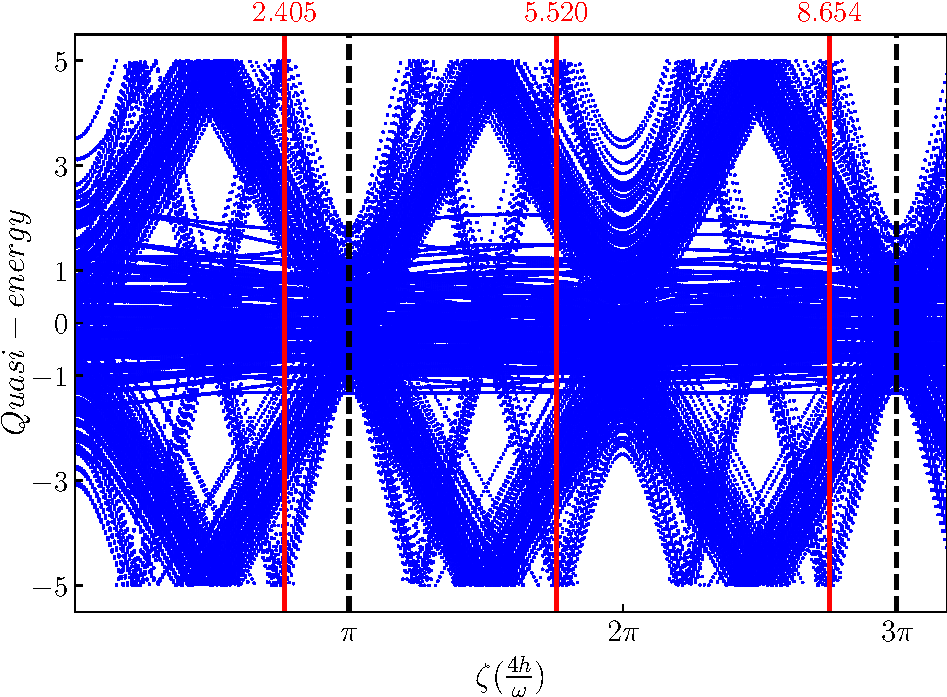
\includegraphics[width=8.3cm]{quasienergy_8.pdf}	
		\caption{Floquet quasi-energy evaluated numerically for the exact Hamiltonian for the one dimensional spin-1/2 spin chain which constitutes a DTC-ferromagnetic-chimera, is plotted for different $\frac{4h}{\omega}$ where $h$ and $\omega$ are drive amplitude and frequency for N = 8 with strong spin coupling interaction. The quasi-energy level repulsion is found (vertical black dashed lines) to be minimum at $(2n+1)\pi$, $n=0,1,2\dots$ The vertical red solid lines represent the roots of Bessel's function of zeroth order i.e. DL points.}
		\label{Fig:quasienergy}
	\end{figure}
	
	Furthermore, when the ratio $({4h}/{\omega}) = (2n+1)\pi$ with $n = 0,1,2\dots$, regions A and B become decoupled even at $\epsilon_A \neq 0$. To see the $h$ and $\omega$ dependency, we numerically obtain the Floquet quasi-energy by diagonalizing the 2T-effective Hamiltonian with $N=8$ and $\epsilon_A=0.03$. Its quasi-energies with different parameters $\zeta( = {4h}/{\omega})$ are plotted in Fig.~\ref{Fig:quasienergy}. The distribution of the quasi-energy exhibits a regular periodic pattern confined in a Brillouin zone in $[-\frac{\pi}{2T}, \frac{\pi}{2T}]$~\cite{dutta2014}. The quasienergy level repulsion is the minimum at each odd integer multiple of $\pi$ in  $\zeta$'s. This is in agreement with the analytical expression in Eq.\eqref{eq:floq_eff3} that a minimum in the eigenvalue of $H^{\mathrm{eff}}$ occurs at $\zeta = (2n+1)\pi$ with $n=0,1,2\dots$.\, at which two regions A and B are completely decoupled even at $\epsilon_A \neq 0$. In contrast, when $0 < \epsilon_A \ll 1 $ and at the DL point, i.e., $\frac{4h}{\omega}$ is one of the roots of $\mathcal{J}_0$, as we have considered in the previous section, now the regions A and B are weakly coupled which is proportional to $\epsilon_A$. 	
	
	\section{\label{sec:level4}Regional  Magnetization \& Entanglement entropy}
	
	\subsection{\label{sec:level42} Regional Magnetization}
	The relative \textit{regional} nature of a segmented spin system can be better comprehended through the analysis of regional magnetization. The concept of regional magnetization, $\displaystyle M^z_{A/B}=\frac{2}{N}\sum_{i\in{A/B}}\expval{\hat{\sigma}^z_i(t)}$~\cite{sakurai_phys_nodate}, pertains to the magnetization exhibited by distinct sections of the system.
	\begin{figure}
		\centering
		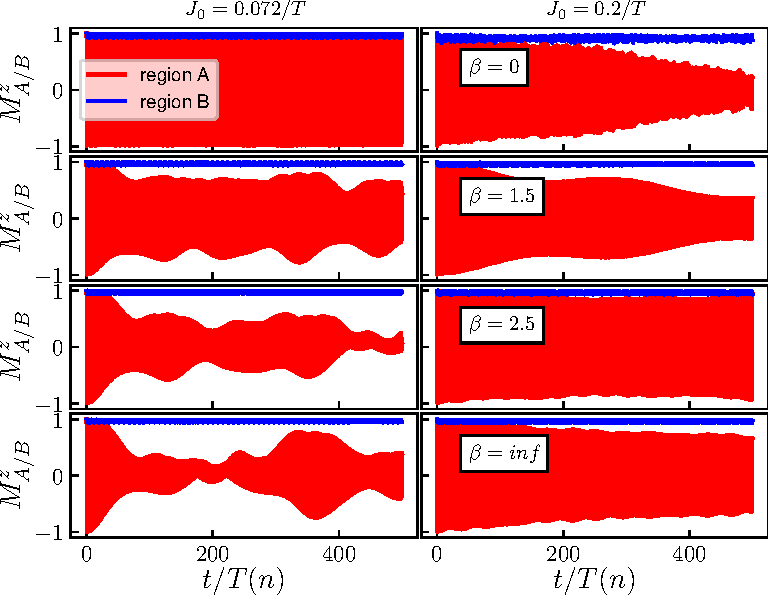
\includegraphics[width = 8cm]{clean_J_strong_MzAB_betas.pdf}
		\caption{Regional magnetization $M^z_{A/B}$ of spins of region A and B for weak spin-coupling (left panels) and strong spin-coupling(right panels) for different spin interactions defined by $\beta$'s up to 500T.}
		\label{Fig:regiogionalmag}
	\end{figure}
	The numerically simulated long time(500T) regional magnetization at region A and region B for both weak and strong spin coupling for different spin interactions are plotted in Fig.~\ref{Fig:regiogionalmag}. For both cases, weak($J_0=0.072/T$) and strong($J_0=0.2/T$) spin interactions are considered at the DL point. In region-B,  $M^Z_B$ is unity throughout time for both types of spin coupling. $M^Z_A$ exhibits differently. At weak coupling, $M^Z_A$ persists for a long time only for long-range ($\beta=0$) interaction, but at other ranges, it dissolves in due course of time. At strong coupling, $M^Z_A$ melts due course of time for all types of spin interactions.
	
	\subsection{\label{sec:level41} Entanglement Entropy}
	In the above sub-section, we have seen the macroscopic quantity (regional magnetization) to investigate the chimera order in our model. In this sub-section, to investigate microscopic aspects, we consider entanglement entropy (EE), which is widely used to measure the entanglement of a quantum state. It offers significant insights into quantum correlations and information storage capacities. The entanglement entropy, $S_{AB}$ between regions A and B can be mathematically expressed by the von Neumann entropy~\cite{bayat_entanglement_2022,mendes-santos_measuring_2020} of the reduced density matrix (RDM).   If the density matrix of the pure state $\ket{\psi}$ is $\rho = \ketbra{\psi}$, and the RDM for regions A or B are defined as $\rho_A$ or $\rho_B$ respectively, then the EE is given by,
	\begin{equation} 
		S_{AB} = -\Tr[\rho_A log(\rho_A)] = -\Tr[\rho_B log(\rho_B)].
		\label{eq:vonentrop}
	\end{equation}	
	\begin{figure}
		\begin{center}
			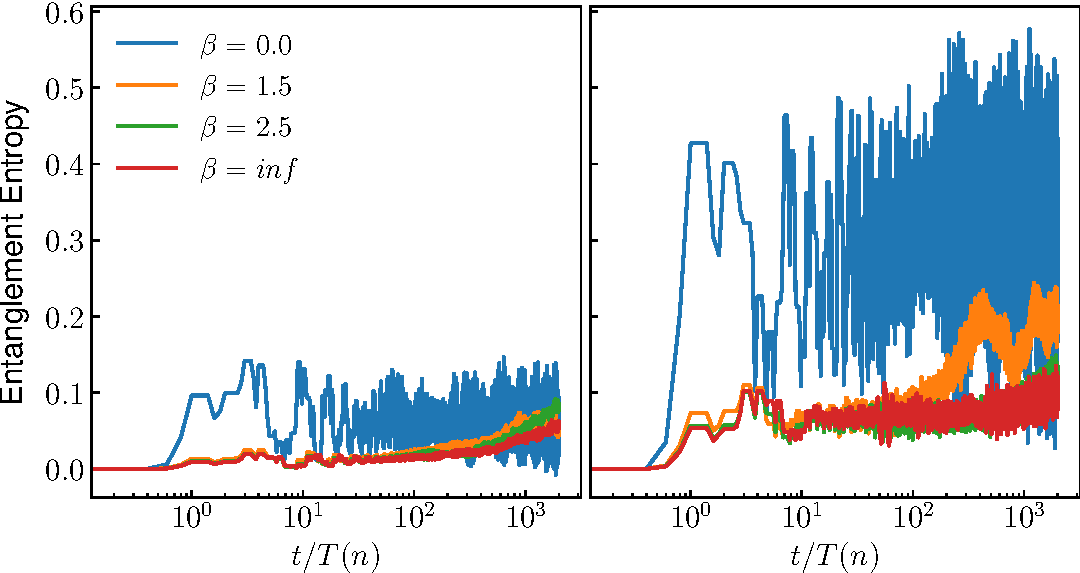
\includegraphics[width=8.5cm]{entangEntrp.pdf}
		\end{center}
		\caption{Entanglement Entropy has been computed at the DL point, considering weaker (left panel) and stronger (right panel) spin exchange couplings. The spin-spin coupling interaction in $\hat{H}_2$ during $T_2$ leads to the onset of a rise in EE. The growth rate of the subject in question remains notably slow, persisting even up to 2000 T.}
		\label{Fig:entangle}
	\end{figure}
	
	We have considered that initially in the spin chain, all of the spins are up. The corresponding density matrix is utilized to evaluate the EE numerically for a total time of 2000T and  plotted in Fig.~\ref{Fig:entangle} for both weak and strong spin-spin interactions. The EE is found to start rising from the onset of $T_2$ from where the spin-spin interaction $\textit{i.e.}$  $\displaystyle \sum_{ij}J_{ij}\hat{\sigma}^y_i\hat{\sigma}^y_j$ starts acting on the spin chain. The EE is found to rise very slowly, even after a sufficiently long time. It has underlying system dynamics that depends on coupling and spin rotation parameters. The coupling strength term of regional spins is kept strong. This prevents the relaxation of regional magnetization. The EE is found to rise faster in strong spin exchange coupling in comparison to weak spin exchange coupling. In Eq.\eqref{eq:floq_eff3} the coupling part of the effective Hamiltonian is proportional to the rotational error($\epsilon_A$), which is considered very small in value. This suppresses the interaction between regions A and B, which results in a small rise in the EE even after a long time period. Thus, a relatively small amount of information is shared between two regions through their inter-coupling.
	
	\section{\label{sec:level6} Robustness against Additional Static field}
	
	
	The enduring stability of the DTC-DMBL chimera is notably influenced by the drive parameters $h$ and $\omega$ in $\hat{H}_2$. The chimera order weakens even with a slight departure from the DL point. This prompts the question of how the chimera resists additional external fields, even when operating precisely at the DL point.
	
	To investigate the robustness of chimera order, we have introduced a static field $\displaystyle \hat{V}(\hat{\sigma}^\gamma) =\gamma \sum_{i=1}^{N} (\hat{\sigma}^x_i + \hat{\sigma}^y_i)$ in addition to the spin-flip operations in $\hat{H_1}$ and spin-spin interacting term along with transverse filed in $\hat{H}_2$, such that the additional static field acts on the system for the entire time period. We considered the drive parameters($h$, $\omega$) corresponding to DL points.
	\begin{figure}
		\begin{center}
			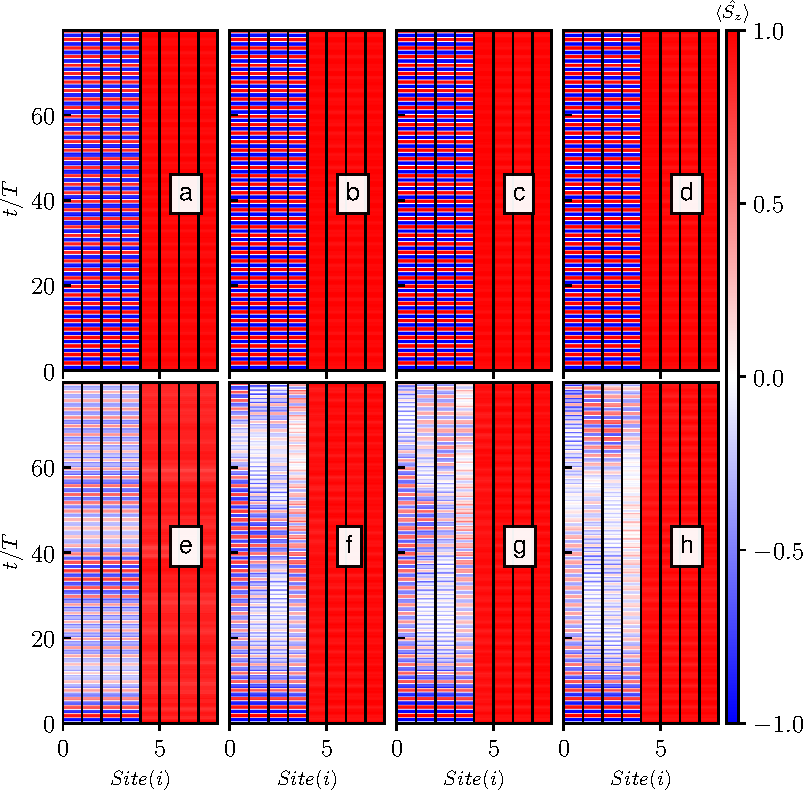
\includegraphics[width=8.5cm]{robustness_N_8.pdf}
		\end{center}
		\caption{Weak (top panel) and strong (bottom panel) additional static fields defined by $\gamma = J_0^s/5, J_0^s$ respectively, are applied in addition to the strong spin coupling interaction and transverse field at different spin-spin interaction ranges defined by $\beta = 0.0 (a,e), 1.5(b,f), 2.5(c,g), \infty(d,h)$. Local magnetization for each site(i) is plotted for 80 T.}
		\label{Fig:robustness}
	\end{figure}
	We have investigated for strong($\displaystyle \gamma= J_0^s=0.2/T$) and relatively weak ($\displaystyle \gamma= J_0^s/5=0.2/5T$) additional static fields. The numerical findings are presented in Fig.~\ref{Fig:robustness}. At weak $\gamma$, the spin-spin interaction dominates over the static field and dynamical localization persists, which results in stable DTC chimera. However, at a higher value of $\gamma$, the static field surpluses the exchange interaction among spins resulting in melting in  the DTC phase after a few time periods. At large times, a \textit{thermal-MBL} chimera phase manifests. Hence, a DTC-ferromagnetic chimera for a one-dimensional spin-1/2 chain can be realized that is robust against an additional external static field.	
	
	
	\section{\label{sec:level7} Discussion and Conclusion}
	
	We have found DTC-DMBL-chimera on a  disorder-free spin-1/2 chain by applying spin-flip operations regionally (with two regions labeled `A' and `B') and, afterward, a global dynamical localization by application of  a high-frequency drive. The weak spin coupling interaction is found to fail to persist in the DTC phase for all interactions except for long-range interaction. A strong spin exchange coupling interaction influences spins to resist relaxation in system dynamics, which yields a stable DTC phase regionally for a sufficiently long time for all types of spin-spin interactions. The stability of DTC in region A depends on the stability of DMBL in region B. The long-range spin interaction is fascinatingly robust against the exchange energy per spin. Long-range interaction enables DTC-DMBL-chimera at both weak and strong coupling interactions. We investigated tuning the spin rotational error at region A and found that at DL points, chimera can persist only at small rotational error $\epsilon_A$. In the effective Floquet Hamiltonian in Eq.~\ref{eq:floq_eff3} the inter-region interaction term is proportional to the spin rotation error $\epsilon_A$. At large $\epsilon_A$ there is higher coupling in between both the regions, which leads to DTC melting immediately for all interactions except for long-range. 
	
	An additional external static field is applied to investigate numerically the robustness of chimera against static perturbations. At small perturbations, the system is found to be robust by retaining the DTC phase in region A for a long time, while at higher perturbations, the system is no longer robust and the DTC melts immediately for all types of spin-spin interactions. The effective Flouquet Hamiltonian depicts time period doubling at the reversal of global ferromagnetic order in the spin chain, which is supported by the exact numerics. The entanglement entropy rises at a very slow rate for both weak and strong regional spin interactions. Thus, the whole system is prevented from thermalization even when the DTC phase is dissolved in region A. This property can be utilized as quantum memory in applications. The proposed model and dynamics can be realized experimentally in trapped ions~\cite{sakurai_phys_nodate, Friedenauer2008}.
	
	In summary, we investigated the factors that contribute to the stability of the DTC-DMBL-chimera order. Long-range spin interaction is found to be the most suitable choice to construct DTC-DMBL-chimera where at DL points, other ranges of spin-spin interactions also contribute. Our analysis focuses on different types of spin-spin interaction defined by the power-law decay rule, the applied regional spin rotational error, the strength of spin-coupling interactions, the applied additional external static field, and periodic drive parameters. These variables are crucial in determining the stability of the chimera order.\\
	
	
\begin{acknowledgments}
	MR thankfully acknowledges The University of Burdwan for support via state-funded fellowship. AR acknowledges support from the University Grants Commission (UGC) of India, via BSR Startup Grant No. F.30-425/2018(BSR), also from the Science and Engineering Research Board (SERB, Govt. of India) Core Research Grant No. CRG/20l8/004002.
\end{acknowledgments}
	
	%%%%%%%%%%%%%%%%%%%%%%%%%%%%%%%%%%%%%%%%%%%%%%%%%%%%%%%%%%%%%%%%%%%%%%%
	% Bibliography
	%
	%
	\bibliographystyle{apsrev4-2}
	\bibliography{chimera}% Produces the bibliography via BibTeX.
	%
	%
	%%%%%%%%%%%%%%%%%%%%%%%%%%%%%%%%%%%%%%%%%%%%%%%%%%%%%%%%%%%%%%
	%Appendix
	\newpage
	\clearpage
	\appendix
	\onecolumngrid
	\section{ DMBL in $T_2$ time interval}
	
	We have considered a spin-1/2 chain consisting of N numbers of spins, which  incorporates Heisenberg interaction following the power law decay rule. The spin chain is considered to be divided into two regions, A and B. In the first half of the time period ($T_1$), a spin flip operation takes place in region A. In the second half of the time period ($T_2$), the spin chain is driven by a global sinusoidal periodic drive \textit{s.t.} $h_D = -h\sin(\omega t)$ as shown in fig \ref{Fig:time_distribution}. This drive is controlled in such a way that in $T_2$, the system is localized by system dynamics.
	
	The Hamiltonian in $T_2$ is $\displaystyle \hat{H}_2(t) = \hbar\sum_{i>j} J_{ij}\hat{\sigma}^y_i\hat{\sigma}^y_j - \hbar h \sin(\omega t) \sum_i \hat{\sigma}^z_i$.
	Where $i$ and $j$ are the sites of spins. $J_{ij} = \frac{J_0}{|i-j|^\beta}$ is the Heisenberg interaction term which incorporates the interaction between the spins at positions  $i$ and $j$ for a power law decay with an exponent $\beta$. 
	The time evolution operator is found to be,
	\begin{equation}
		\hat{W}(t) = \exp \bigg[-\frac{i}{\hbar}\int_{\frac{T}{2}}^{\frac{T}{2}+t} (-h \sin(\omega t'))dt' \hbar\sum_i\hat{\sigma}^z_i\bigg]
		=\prod_{i} \exp\big[-i \hat{\sigma}^z_i\theta(t)\big],
	\end{equation}
	where, $\displaystyle \theta (t) = h\int_{\frac{T}{2}}^{\frac{T}{2}+t}  (-\sin(\omega t')dt') =\frac{h}{\omega}(1-\cos(\omega t))$.
	Now, the Hamiltonian in moving frame can be transformed to\cite{haldar_statistical_2022},
	\begin{align}
		\hat{H^{mov}} &= \hat{W}^\dagger(t) \hat{H}(t) \hat{W}(t)- i \hat{W}^\dagger(t) \partial_t \hat{W}(t) \nonumber\\
		&= \hat{W}^\dagger(t) H_0 \hat{W}(t)\nonumber\\
		&= \prod_{i} \exp\big[-i\hat{\sigma}^z_i \theta(t)\big] \big[\hbar\sum_{ij}J_{ij}\hat{\sigma}^y_i\hat{\sigma}^y_j\big] \exp\big[ i\hat{\sigma}^z_i \theta(t)\big]\nonumber\\
		&= \hbar\sum_{ij} J_{ij} e^{-i\hat{\sigma}^z_i \theta(t)} e^{-i\hat{\sigma}^z_j  \theta(t)}\Big(\hat{\sigma}^y_i\hat{\sigma}^y_j\Big)e^{i\hat{\sigma}^z_i \theta(t)} e^{i\hat{\sigma}^z_j \theta(t)}\nonumber\\
		&= \hbar\sum_{ij} J_{ij} \Big(\hat{\sigma}^y_i\hat{\sigma}^y_j\Big)e^{i2\hat{\sigma}^z_i \theta(t)} e^{i2\hat{\sigma}^z_j \theta(t)}\nonumber\\
		&= \hbar\sum_{ij} J_{ij} \Big(\hat{\sigma}^y_i\hat{\sigma}^y_j\Big) \Big(\cos^2(2\zeta) -\hat{\sigma}^z_i\hat{\sigma}^z_j \sin^2(2\zeta) + i (\hat{\sigma}^z_i + \hat{\sigma}^z_j)\cos(2\zeta)\sin(2\zeta)\Big).
		\label{eq:hmovap1}
	\end{align}
	Here, we have considered, $\zeta = \frac{h}{\omega}(1-\cos(\omega t))$ and used the expression, $\exp(\mathbbm{1} \cos(a) + i (\hat{n}.\vec{\sigma})\sin(a))$. 
	Thus one can get,
	\begin{multline}
		\cos(2\zeta) =\cos(\frac{2h}{\omega})\Bigg(J_0\Big(\frac{2h}{\omega}\Big) + 2\sum_{n=1}^\infty (-1)^n J_{2n}\Big(\frac{2h}{\omega}\Big)\cos(2n\omega t)\Bigg)\\ + \sin(\frac{2h}{\omega})\Bigg(-2\sum_{n=1}^\infty (-1)^n J_{2n-1}\Big(\frac{2h}{\omega}\Big)\cos([2n-1]\omega t)\Bigg).
	\end{multline}
	The drive frequency being high, higher-order terms can be neglected. So, we get,  $\displaystyle \cos(2\zeta) = \cos(\frac{2h}{\omega})J_0\Big(\frac{2h}{\omega}\Big)$. Similarly, $\displaystyle \sin(2\zeta) = \sin(\frac{2h}{\omega})J_0\Big(\frac{2h}{\omega}\Big)$. Here we have applied Jacobi Anger expansion which is $e^{i z \cos(\theta)} = \sum_{n=-\infty}^{\infty} \mathcal{J}_n(z) e^{in\theta}$, where $\mathcal{J}$'s are the roots of the Bessel's function of first kind.
	
	\noindent Putting the values in ~\eqref{eq:hmovap1}, the moving frame transformed Hamiltonian becomes,
	\begin{equation}
		\hat{H}^{mov} = \hbar\sum_{ij} J_{ij} \Big(\hat{\sigma}^y_i\hat{\sigma}^y_j\Big)\;J_0\Big(\frac{4h}{\omega}\Big)\Bigg(\cos[2](\frac{2h}{\omega}) -i\Big(\hat{\sigma}^z_i\hat{\sigma}^z_j\Big) \sin[2](\frac{2h}{\omega})+ i (\hat{\sigma}^z_i + \hat{\sigma}^z_j)\cos(\frac{2h}{\omega})\sin(\frac{2h}{\omega})\Bigg).
		\label{eq:hmovfinal}
	\end{equation}
	At the roots of Bessel's function of the first order, the rotating frame Hamiltonian($\hat{H}^{mov}$) vanishes. Eq.\eqref{eq:hmovfinal} describes the necessary and sufficient condition for dynamical localization in $T_2$. At the roots of Bessel's function of the first kind,  which is determined by the system parameters as $\frac{4h}{\omega}$, the transformed Hamiltonian in the moving frame vanishes, which manifests dynamical localization (DL).
	
	\section{\label{sec:appnfloq} Effective Floquet Hamiltonian}
	
	Floquet theory is an efficient methodology for evaluating the behavior of systems that undergo periodic driving by converting the time-varying problem into a time-invariant one. The Hamiltonian for a periodically driven system can be written as,
	\begin{equation*}
		\hat{H}(t) = \hat{H}_0 + \varepsilon \hat{H}_1(t)
	\end{equation*}
	The corresponding unitary evolution operator can be found from $\displaystyle{i\hbar \partial_t \hat{U}(t) = \hat{H}(t) \hat{U}(t)}$. Here $\displaystyle{\hat{U}(t) = \hat{U}(t+ nT)}$. For one time period T, the unitary operator $\displaystyle \hat{U}(T) = \hat{\mathcal{F}}$ is called the Floquet operator which is related to Floquet effective Hamiltonian ($\hat{H}_F$) as $\hat{U}(t) = \exp[-\frac{i}{\hbar}\hat{H}_F T]$~\cite{Eckardt_2015}. $\hat{H}_F\,(=H^\mathrm{eff})$ is derived from the original time-dependent Hamiltonian through a suitable transformation. Floquet Magnus expansion (FM) provides a systematic approach for analyzing the dynamics of quantum systems subjected to high-frequency periodic driving. By calculating successive terms in the expansion, one can derive an effective Hamiltonian that captures the essential physics of the system and allows for a deeper understanding of its behavior. $\hat{H}_F$ can be expanded as~\cite{Sen_2021},	
	\begin{align}
		\hat{H}_F &= \sum_{n=0}^{\infty} H_F^{(n)}\nonumber\\
		H_F^{(0)} &= \frac{1}{T} \int_{t_0}^{T+t_0} dt H(t), \nonumber\\
		H_F^{(1)} &= \frac{1}{2!\hbar(i)T} \int_{t_0}^{T+t_0} dt_1  \int_{t_0}^{t_1} dt_2 [H(t_1), H(t_2)]\nonumber\\
		H_F^{(2)} &= -\frac{1}{3!\hbar^2 T^3} \int_{t_0}^{T+t_0} dt_1  \int_{t_0}^{t_1} dt_2 \int_{t_0}^{t_2} dt_3([H(t_1),[H(t_2), H(t_3)]] + [H(t_3),[H(t_2), H(t_1)]])
		\label{eq:app:mageff}
	\end{align} 
	Here each order `$n$' of the previous expansion in Eq.~\ref{eq:app:mageff} is hermitian~\cite{haldar_statistical_2022}.
	
	The proposed spin chain in Eq.\eqref{eq:cleanham}undergoes two time periods to construct a DTC. To obtain Floquet equation for the Hamiltonian in Eq.~\ref{eq:cleanham}, Flqouet operator $\hat{\mathcal{F}}$ is acted twice on the Hamiltonian from time $t=0$ to $t=2T$ as,
	\begin{align*}
		\hat{\mathcal{F}}^2 &= \exp\Big(-\frac{i}{\hbar}\hat{H}_{\epsilon_A, 2T}^{\mathrm{eff}}2T\Big)\\ 
		&= \mathcal{T}\exp\Big(-\frac{i}{\hbar}\int_{\frac{3T}{2}}^{2T}\hat{H}_2 dt\Big)
		\exp\Big(-\frac{i}{\hbar}\hat{H}_1T_1\Big)\mathcal{T}\exp\Big(-\frac{i}{\hbar}\int_{\frac{T}{2}}^{T}\hat{H}_2 dt\Big)\exp\Big(-\frac{i}{\hbar}\hat{H}_1T_1\Big).
		\label{}
	\end{align*}
	Here $\mathcal{T}$ is the time-ordered exponential. The effective Floquet coefficients can be evaluated as given below,	
	\begin{align}
		H_F^{(0)} &= \frac{2}{T} \int_{\frac{T}{2}}^{T} dt H(t) = \frac{2}{T} \int_{\frac{T}{2}}^{T} dt \Bigg[\hbar\sum_{i\neq j} J_{ij} \hat{\sigma}^y_i \hat{\sigma}^y_j -\hbar h\sin(\omega t) \sum_i\hat{\sigma}^z_i\Bigg]= \hbar\sum_{i\neq j} J_{ij} \hat{\sigma}^y_i \hat{\sigma}^y_j + \frac{4h\hbar}{T \omega}\sum_i\hat{\sigma}^z_i,
	\end{align}	
	\begin{align}
		H_F^{(1)} &= \frac{1}{2!(i)\hbar} \frac{2}{T} \int_{\frac{T}{2}}^{T} dt_1  \int_{\frac{T}{2}}^{t_1} dt_2 [H(t_1), H(t_2)]\nonumber\\
		&= \frac{1}{2!(i)\hbar} \frac{2}{T}\int_{\frac{T}{2}}^{T} dt_1 \int_{\frac{T}{2}}^{t_1} dt_2\Bigg[2i\hbar\sum_{ij}^{}J_{ij}\hat{\sigma}^x_i\hat{\sigma}^y_j\Big\{h(t_2) -h(t_1)\Big\}\Bigg]\nonumber\\
		&= 0
	\end{align}	
	and,
	\begin{equation}
		H_F^{(2)} = -\frac{1}{3!\hbar^2 (T/2)^3} \int_{\frac{T}{2}}^{T} dt_1  \int_{{\frac{T}{2}}}^{t_1} dt_2 \int_{\frac{T}{2}}^{t_2} dt_3([H(t_1),[H(t_2), H(t_3)]] + [H(t_3),[H(t_2), H(t_1)]])= 0.    
	\end{equation}
	Thus the effective Hamiltonian in the interval $T_1\equiv[\frac{T}{2}, T]$ found to be,	
	\begin{equation}
		H^{\mathrm{eff}}\vert_{\frac{T}{2}, T} =  \hbar\sum_{i\neq j} J_{ij} \hat{\sigma}^y_i \hat{\sigma}^y_{j} + \frac{4h\hbar}{T \omega}\sum_i\hat{\sigma}^z_i.
	\end{equation} 	
	Similarly, the effective Hamiltonian for time interval $T_2\equiv[\frac{3T}{2}, 2T]$ is found as,	
	\begin{equation}
		H^{\mathrm{eff}}\vert_{\frac{3T}{2}, 2T} = \hbar\sum_{i\neq j} J_{ij} \hat{\sigma}^y_i \hat{\sigma}^y_{j} + \frac{4h\hbar}{T \omega}\sum_i\hat{\sigma}^z_i.
	\end{equation} 
	Let us consider, $\epsilon_A \neq 0$ and $\epsilon_B=1$. Also, we consider $\displaystyle \hat{V}_{\epsilon_A} = \exp\Big(\frac{i\epsilon_A \pi}{2}\sum_{l\in A}\hat{\sigma}^x_l\Big)$  and $\displaystyle \hat{\theta}_l = 2 \Big(\sum_{m \in B}J_{lm}\hat{\sigma}^y_m \frac{T}{2} \Big)$ which denotes a rotation acting on operator $\hat{\sigma}^y_l$, also we have contracted all the terms contributed from only region B. We consider, $\displaystyle {H}_B = \Big(\sum_{l,m\in B} J_{lm} \hat{\sigma}^y_l\hat{\sigma}^y_m + \frac{4h}{\omega T}\sum_{m \in B}\hat{\sigma^z_m}\Big)$. So, we can write,		
	\begin{multline}
		\mathcal{T}\exp(-\frac{i}{\hbar}\int_{\frac{T}{2}}^{T} \hat{H}_2 dt) = \exp\Bigg[-i \Big[ \sum_{l,m\in A}J_{lm} \hat{\sigma}_l^y\hat{\sigma}_m^y +\sum_{l,m\in B}J_{lm}
		\hat{\sigma_l^y}\hat{\sigma_m^y}-\sum_{\substack{%
				l \in A,\\
				m \in B\hfill}} J_{lm}\hat{\sigma}^y_l\hat{\sigma}^y_m\\+\frac{4h}{\omega T}\Big\{ -\sum_{l\in A}^{}\hat{\sigma}^z_l + \sum_{m\in B}^{}\hat{\sigma}^z_m\Big\}\Big]\frac{T}{2}\Bigg],
	\end{multline}	
	and, $\displaystyle 
	\exp\Big(-\frac{i}{\hbar} \hat{H}_1 T_1\Big) = \exp\Bigg[\frac{-i(1-\epsilon_A)\pi}{2}\sum_{l \in A}\hat{\sigma}^x_l\Bigg].$
	Putting these values in the Floquet operator equation can be written as,    	
	\begin{align}
		\hat{\mathcal{F}}^2 
		=& \exp\Bigg[-i \Big[ \sum_{l,m\in A}J_{lm} \hat{\sigma}^y_l\hat{\sigma}^y_m\frac{T}{2} +\sum_{l,m\in B}J_{lm} \hat{\sigma}^y_l\hat{\sigma}^y_m\frac{T}{2}+\sum_{\substack{%
				l \in A,\\
				m \in B\hfill}} J_{lm}\hat{\sigma}^y_l\hat{\sigma}^y_m\frac{T}{2} +\frac{2h}{\omega }\Big\{ +\sum_{l\in A}^{}\hat{\sigma}^z_l + \sum_{m\in B}^{}\hat{\sigma}^z_m\Big\}\Big]\Bigg] \hat{V}_{\epsilon_A} \nonumber\\
		& \hspace{1 cm}\exp\Bigg[-i \Big[ \sum_{l,m\in A}J_{lm} \hat{\sigma}^y_l\hat{\sigma}^y_m\frac{T}{2} +\sum_{l,m\in B}J_{lm} \hat{\sigma}^y_l\hat{\sigma}^y_m\frac{T}{2}-\sum_{\substack{%
				l \in A,\\
				m \in B\hfill}} J_{lm}\hat{\sigma}^y_l\hat{\sigma}^y_m\frac{T}{2} +\frac{2h}{\omega}\Big\{ -\sum_{l\in A}^{}\hat{\sigma}^z_l + \sum_{m\in B}^{}\hat{\sigma}^z_m\Big\}\Big]\Bigg] \hat{V}_{\epsilon_A}\nonumber\\
		=& \exp\Bigg[-i \sum_{l,m\in A}J_{lm} \hat{\sigma}^y_l\hat{\sigma}^y_m\frac{T}{2}\Bigg] \exp\Bigg[-i\Big(\frac{2h}{\omega } \sum_{l\in A}^{}\hat{\sigma}^z_l + \sum_{l \in A}\frac{\hat{\theta}_{l}}{2}\hat{\sigma}^y_l\Big)\Bigg]\nonumber\\ 
		&\hspace{3cm} \hat{V}_{\epsilon_A} \exp\Bigg[i \Big(\sum_{l \in A}\frac{\hat{\theta}_{l}}{2}\hat{\sigma}^y_l + \frac{2h}{\omega} \sum_{l\in A}^{}\hat{\sigma}^z_l\Big)\Bigg] \exp\Bigg[-i\sum_{l,m\in A}J_{lm} \hat{\sigma}^y_l\hat{\sigma}^y_m\frac{T}{2}\Bigg] \exp\big[-i H_B T\big]\hat{V}_{\epsilon_A}\nonumber\\
		=& \exp\Bigg[-i 2 \sum_{l,m\in A}J_{lm} \hat{\sigma}^y_l\hat{\sigma}^y_m\frac{T}{2}\Bigg]\exp\Bigg[\frac{i \epsilon_A \pi}{2}\sum_{l\in A}\Big\{\hat{\sigma}^x_l \cos(\hat{\theta}_l)\cos(\frac{4h}{\omega})\nonumber\\
		&\hspace{7cm}+ \hat{\sigma}^y_l \cos(\hat{\theta}_l)\sin(\frac{4h}{\omega})-\hat{\sigma}^z_l \sin(\hat{\theta}_l)\Big\}\Bigg] \exp\big[-i H_B T\big]\hat{V}_{\epsilon_A}\nonumber\\
		=&exp\Bigg[-i 2\sum_{l,m\in A}J_{lm} \hat{\sigma}_l^y\hat{\sigma}_m^y\frac{T}{2}\Bigg] \exp\Big(\frac{i\epsilon_A \pi}{2}\sum_{l\in A}\hat{\sigma^x_l}\Big) \exp\Bigg[\frac{i \epsilon_A \pi}{2}\sum_{l\in A}\Big\{\hat{\sigma}^x_l \cos(\hat{\theta}_l)\cos(\frac{4h}{\omega})\nonumber\\
		&\hspace{ 7cm}  +\hat{\sigma}^y_l \cos(\hat{\theta}_l)\sin(\frac{4h}{\omega})-\hat{\sigma}^z_l \sin(\hat{\theta}_l)\Big\}\Bigg]\exp\big[-i H_B T\big]\nonumber\\
		=&\exp\Bigg[-i2\sum_{l,m\in A}J_{lm}\hat{\sigma}^y_l\hat{\sigma}^y_m \frac{T}{2}\Bigg] \exp\Bigg[-i\epsilon_A \pi \sum_{\substack{l,m \in A\\l\neq m}}J_{lm} \hat{\sigma}^z_l\hat{\sigma}^y_m\frac{T}{2}\Bigg] \exp\Bigg[\frac{i \epsilon_A \pi}{2}\sum_{l\in A}\Bigg\{\hat{\sigma}^x_l\Bigg( \cos(\hat{\theta}_l)\cos(\frac{4h}{\omega})+1\Bigg)\nonumber\\
		&\hspace{7cm} +\hat{\sigma}^y_l \cos(\hat{\theta}_l)\sin(\frac{4h}{\omega})-\hat{\sigma}^z_l \sin(\hat{\theta}_l)\Bigg\}\Bigg] \exp\big[-i H_B T\big]
		\label{eq:floq_couple1}
	\end{align}
	Now, utilizing the relation $\displaystyle \hat{\mathcal{F}}^2 = \exp\Big(-\frac{i}{\hbar}H^{\mathrm{eff}}2T\Big)$, the effective Floquet hamiltonian can be found as,
	\begin{multline}
		H^{\mathrm{eff}} \approx\frac{\hbar}{2} \sum_{l,m\in A}J_{lm}\hat{\sigma}_l^y\hat{\sigma}_m^y +\frac{\hbar \epsilon_A \pi}{4} \sum_{\substack{l,m\in A\\l\neq m}} J_{lm}\hat{\sigma}^z_l\hat{\sigma}^y_m + \frac{\hbar}{2}\sum_{l,m\in B}J_{lm}\hat{\sigma}_l^y \hat{\sigma}_m^y + \frac{h\hbar}{\pi}\sum_{m \in B}\hat{\sigma}^z_m \\ -\frac{\hbar \pi \epsilon_A}{4T}\sum_{l\in A}\Bigg[\hat{\sigma}^x_l \Bigg(\cos(\hat{\theta}_l)\cos(\frac{4h}{\omega})+1 \Bigg) + \hat{\sigma}^y_l \cos(\hat{\theta}_l)\sin(\frac{4h}{\omega})-\hat{\sigma}^z_l \sin(\hat{\theta}_l)\Bigg].
		\label{eq:app:nfloq_eff3}
	\end{multline}
	At high frequency drive $T\rightarrow 0$ which makes $\hat{\theta}_l \rightarrow 0$. Thus  Eq.\eqref{eq:app:nfloq_eff3} becomes dependent on ratio $\frac{4h}{\omega}$ when $\epsilon_A \neq 0$.
	
	
	
\end{document}